\documentclass[12pt]{article}
\usepackage[utf8]{inputenc}
\usepackage{graphicx}
\usepackage{amsmath} % for mathematical symbols
\usepackage{amssymb} % for \mathbb command
\usepackage[backend=biber,style=numeric]{biblatex}
\graphicspath{ {images/} }
\addbibresource{references.bib} % Specify the name of your .bib file

\title{
{\textbf{Technical University of Košice}}\\
\vspace{12pt}
{\large \textbf{Faculty of Mining, Ecology, Process Control\\ and Geotechnologies}}\\
\vspace{12pt}
{\large Institute of Control and Informatization of Production Processes}\\
\vspace{64pt}
{\textbf{Process Theory}}\\
}
\author{Ing. Ales Jandera}
\date{10. May 2024}

\begin{document}

\maketitle

\newpage

\tableofcontents

\newpage

\section{Introduction}
Process theory from a cybernetics viewpoint involves the study of systems,
especially looking at how systems process information and maintain control
through feedback mechanisms. Cybernetics, founded by Norbert Wiener, is
fundamentally concerned with communication and control in animals, humans,
and machines. It emphasizes the essential roles of feedback, regulation,
and dynamics in systems.\\
\\
\textbf{Core Concepts of Process Theory in Cybernetics}\\
\\
Feedback Loops divided to \textbf{Negative Feedback} is used to reduce
discrepancies between the actual state and desired state,
stabilizing the system. It is prevalent in both biological systems 
(like homeostasis in human bodies) and mechanical systems (such as
thermostats) and \textbf{Positive Feedback} amplifies deviations or changes,
potentially leading to exponential growth or runaway effects. It's often
seen in processes like population growth or economic bubbles but needs
to be carefully managed to prevent instability.\\
\\
\textbf{Homeostasis} refers to the ability of a system to maintain
internal stability despite external changes. In cybernetics, this
concept is crucial for understanding how biological organisms and even
social systems preserve their integrity and function.\\
\\
Cybernetics studies how systems adapt to their environments and learn
from interactions. This involves adjusting internal mechanisms based on
external changes, a principle applicable to both living organisms and
artificial intelligence systems.\\
\\
Systems can develop structures and patterns internally without specific,
external commands or controls. This emergent behavior is central to
understanding complex systems in cybernetics, from neural networks to
social systems.\\
\\
\textbf{Control Theory} a branch closely related to cybernetics, focusing
on how to direct systems toward desired states. It involves designing
control systems that can measure the current state, compare it to a
target or set point, and act to minimize any deviations.\\
\\
\textbf{System Dynamics} involves the study of how systems evolve over
time, considering the interdependencies and feedback loops that affect
their behavior. This includes looking at both linear and non-linear
dynamics, which can exhibit very different behaviors under changing
conditions.\\
\\
\textbf{Applications and Implications}\\
\begin{itemize}
\item Robotics and Automation understanding process theory in cybernetics helps in designing more effective and autonomous robots that can interact dynamically with their environments.
\item Biological Sciences offers insights into physiological processes and ecosystems' dynamics.
\item Management and Organization helps in designing better organizational structures and management practices that can adapt and thrive in changing environments.
\item Artificial Intelligence influences the development of algorithms that can learn and adapt, enhancing their decision-making capabilities.
\end{itemize}
\section{Methods}
%
Studying cybernetic processes involves a multidisciplinary approach that
merges concepts from engineering, mathematics, biology, and social
sciences to understand control and communication in systems. The methods
used to study cybernetics are diverse, reflecting the broad scope of the
field which ranges from theoretical frameworks to practical
implementations.
%
    \subsection{Partial Derivation}
    %
    Partial derivatives are a fundamental concept in calculus, particularly in
    the field of multivariable calculus. They describe how a function
    changes as one of its variables changes, holding the other variables
    constant. This is essential in many applications across physics,
    engineering, economics, and more, where functions often depend on more
    than one variable.\\
    \\
    \textbf{Basic Concept}\\
    \\
    Suppose you have a function \( f \) that depends on two variables,
    \( x \) and \( y \). The partial derivative of \( f \) with respect
    to \( x \) measures how \( f \) changes as \( x \) changes, while
    keeping \( y \) constant. Similarly, the partial derivative of \( f \)
    with respect to \( y \) measures how \( f \) changes as \( y \) changes,
    while keeping \( x \) constant.\\
    \\
    \textbf{Notation}\\
    \\
    Partial derivatives can be denoted in several ways. For a function \( f(x, y) \),
    the partial derivative with respect to \( x \) is denoted as:
    \begin{equation}
        \frac{\partial f}{\partial x} \text{ or } f_x
    \end{equation}
    Similarly, the partial derivative with respect to \( y \) is denoted as:
    \begin{equation}
        \frac{\partial f}{\partial y} \text{ or } f_y
    \end{equation}
    \\
    \textbf{Calculating Partial Derivatives}\\
    \\
    If you have a function \( f(x, y) = x^2y + 3xy^3 \), the partial derivatives would be
    calculated as follows:\\
    \begin{enumerate}
    \item Partial Derivative with respect to \( x \)
    \begin{equation}
       \frac{\partial f}{\partial x} = \frac{\partial}{\partial x} (x^2y + 3xy^3)
        = 2xy + 3y^3
    \end{equation}
       Here, \( y \) is treated as a constant, and you differentiate \( x^2y \) and \( 3xy^3 \) with respect to \( x \).
    
    \item Partial Derivative with respect to \( y \)
    \begin{equation}
       \frac{\partial f}{\partial y} = \frac{\partial}{\partial y} (x^2y + 3xy^3)
       = x^2 + 9xy^2
    \end{equation}
       Here, \( x \) is treated as a constant, and you differentiate \( x^2y \) and \( 3xy^3 \) with respect to \( y \).
    \end{enumerate}
    \textbf{Higher-Order Partial Derivatives}\\
    \\
    Partial derivatives can also be extended to higher orders. For example, the second-order
    partial derivatives of \( f \) are:\\
    The second partial derivative of \( f \) with respect to \( x \) twice:
    \begin{equation}
        \frac{\partial^2 f}{\partial x^2}
    \end{equation}
    The second partial derivative of \( f \) with respect to \( y \) twice:
    \begin{equation}
        \frac{\partial^2 f}{\partial y^2}
    \end{equation}
    The mixed partial derivative first with respect to \( x \) and then with respect to \( y \):
    \begin{equation}
        \frac{\partial^2 f}{\partial x \partial y}
    \end{equation}
    The mixed partial derivative first with respect to \( y \) and then with respect to \( x \):
    \begin{equation}
        \frac{\partial^2 f}{\partial y \partial x}
    \end{equation}
    \\
    \textbf{Applications}\\
    \\
    Partial derivatives are used in various ways, such as:\\
    \\
    \textbf{Gradient vectors}, which are vectors of partial derivatives used in optimization
    problems.\\
    \\
    \textbf{Jacobian matrices} in multivariable transformation, which consist of
    first-order partial derivatives.\\
    \\
    \textbf{Hessian matrices} in optimization, which are matrices of second-order
    partial derivatives used to assess the curvature of multivariable functions.\\
    \\
    Understanding and calculating partial derivatives is crucial for analyzing and predicting
    the behavior of systems that depend on multiple variables, providing a foundation for
    further studies and applications in more complex mathematical, physical, and economic
    models.
    %
    \subsection{Volterra Series}
    %
    The Volterra series~\cite{wiener1958} models the output of a nonlinear system as a functional series,
    where the output depends not only on the current input but also on past inputs, capturing
    the history-dependent behavior of the system. This is crucial for accurately describing
    systems where the output is not merely a direct proportional response to the input.\\
    \\
    Components of the Volterra Series:\\
    \begin{enumerate}
    \item Linear and Nonlinear Kernels of the Volterra series is built up of kernels of
    increasing order that correspond to the system's linear, quadratic, cubic, and
    higher-order responses. Each kernel integrates the product of input values at multiple
    time points, reflecting the combined effects of these inputs over time.
    \item Integration over Time Delays involve the kernels integration over different combinations
    of time delays, representing how past inputs influence the current output.
    This integration makes the model particularly useful for analyzing systems with memory.\\
    \item Expansion Terms series includes terms of increasing complexity, with each
    higher-order term accounting for more complex interactions between input values
    at different times. The first-order kernel represents the linear response, the
    second-order kernel captures pairwise interactions (quadratic nonlinearity), and
    higher-order kernels describe more complex dynamics.
    \end{enumerate}

    \noindent Applications of Voltera Series models are in the \textbf{Signal Processing} where Volterra series
    are used to model and predict nonlinear distortions in signals, such as
    in audio processing or telecommunications, where equipment nonlinearity affects the
    signal integrity then in \textbf{Control Systems} in control theory helps in designing controllers
    that can handle nonlinear dynamics effectively, ensuring stability and performance in
    nonlinear control systems. In the \textbf{Biological Systems} are applied in modeling
    the nonlinear responses of biological systems, such as the neural response functions
    in sensory systems where the output response to stimuli is inherently nonlinear.\\
    \\
    As the order of interaction increases, the computational complexity of the model can
    grow significantly, making higher-order models difficult to manage. Accurately estimating
    the higher-order kernels requires extensive data, and the model may suffer from
    overfitting if not properly regularized or if the data is not sufficient.\\
    \\
    The Volterra series provides a powerful framework for understanding and predicting
    the behavior of nonlinear systems, though its practical application requires careful
    consideration of its complexity and the computational resources available.\\
    \\
    \textbf{Volterra Series Expansion}\\
    \\
    The output \( y(t) \) of a nonlinear system in response to an input \( x(t) \) can be
    expressed as:
    \begin{equation}
        y(t) = h_0 + \sum_{n=1}^{\infty} \int_{-\infty}^\infty \int_{-\infty}^\infty \cdots \int_{-\infty}^\infty h_n(\tau_1, \tau_2, \ldots, \tau_n) x(t-\tau_1) x(t-\tau_2) \cdots x(t-\tau_n) \, d\tau_1 \, d\tau_2 \cdots d\tau_n,
    \end{equation}
    \noindent where, \( h_n(\tau_1, \tau_2, \ldots, \tau_n) \) are the Volterra kernels, which
    are functions characterizing the system's response at different orders of interaction
    between time-shifted inputs. Each kernel \( h_n \) corresponds to the \( n \)-th order
    of nonlinearity in the system's response:\\

    \noindent \( h_0 \) is a constant term, often representing the system's output at zero input.
    \( h_1(\tau_1) \) is the first-order kernel or linear response of the system.
    \( h_2(\tau_1, \tau_2) \) is the second-order kernel, capturing the pairwise nonlinear interactions.
    \( h_3(\tau_1, \tau_2, \tau_3) \)* and higher-order kernels account for increasingly complex interactions.\\
    
    \newpage
    \noindent \textbf{First and Second-Order Kernels}\\
    \\
    For practical applications, the Volterra series is often truncated after a few terms.
    Here's how the first and second-order terms are typically expressed:\\
    \\
    First-order (linear) response:\\
    \begin{equation}
    y_1(t) = \int_{-\infty}^\infty h_1(\tau_1) x(t-\tau_1) \, d\tau_1
    \end{equation}

    \noindent Second-order (quadratic) response:\\
    \begin{equation}
        y_2(t) = \int_{-\infty}^\infty \int_{-\infty}^\infty h_2(\tau_1, \tau_2) x(t-\tau_1) x(t-\tau_2) \, d\tau_1 \, d\tau_2
    \end{equation}
    %
    \subsection{Backporpagation}
    %
    Backpropagation is a method commonly used in artificial neural networks to train the network
    by adjusting the weights of the synapses. This adjustment is done by comparing the network's
    actual output to the desired output and updating the weights accordingly, allowing the network
    to learn and improve its performanceover time. Backpropagation is a fundamental algorithm in
    the field of artificial neural networks~\cite{WOS:000797637800002}. Backpropagation is a
    fundamental algorithm in the field of artificial neural networks, allowing for the training
    and improvement of the network by adjusting the weights of thesynapses based on the error
    between the actual output and the desired output. The algorithm works by propagating the
    error backwards through the network, hence its name "backpropagation"~\cite{WOS:000916261400001}.
    The backpropagation algorithm is a crucial tool in training artificial neural networks.
    It allows for the optimization of network performance by adjusting synapse weights based
    on the error between actual and desired outputs. Furthermore, backpropagation has
    demonstrated its power in optimizing the performance of neural networks by allowing
    psychologists to design networks capable of performing complex computations in
    unexpected ways and uncovering insights from data.\\
    
    \newpage
    \begin{enumerate}
    \item Forward Pass\\
    During the forward pass, the input data is fed through the neural network, and the output
    is computed through successive activations of the network layers.
    For each layer \( l \), the input \( z^{(l)} \) and output \( a^{(l)} \) are computed as follows:
    \begin{equation}
        z^{(l)} = W^{(l)} \cdot a^{(l-1)} + b^{(l)},
    \end{equation}
    \begin{equation}
        a^{(l)} = \sigma(z^{(l)}),
    \end{equation}

    where:\\
    \( W^{(l)} \) is the weight matrix for layer \( l \),\\
    \( b^{(l)} \) is the bias vector for layer \( l \),\\
    \( a^{(l-1)} \) is the output of the previous layer,\\
    \( \sigma \) is the activation function applied element-wise to the input.\\
    \item Backward Pass (Error Backpropagation)\\
    During the backward pass, the gradients of the loss function with respect to the weights and biases of the network are computed using the chain rule of calculus.
    \\
    Compute the output layer error \( \delta^{(L)} \) as the derivative of the loss function with respect to the output activations:
    \begin{equation}
        \delta^{(L)} = \nabla_a L \odot \sigma'(z^{(L)})
    \end{equation}

    Backpropagate the error through the network layers to compute the errors \( \delta^{(l)} \) for each hidden layer:
    \begin{equation}
        \delta^{(l)} = ((W^{(l+1)})^T \cdot \delta^{(l+1)}) \odot \sigma'(z^{(l)})
    \end{equation}
    \item Gradient Descent Update\\
    Use the computed errors to update the weights and biases of the network using gradient descent or its variants. 
    Update the weights and biases of each layer using the gradients of the loss function with respect to the weights and biases:
    \newpage
    \begin{equation}
        \frac{\partial L}{\partial W^{(l)}} = \delta^{(l)} \cdot (a^{(l-1)})^T,
    \end{equation}
    \begin{equation}
        \frac{\partial L}{\partial b^{(l)}} = \delta^{(l)},
    \end{equation}

    where:\\
        \( L \) is the loss function,\\
        \( \odot \) denotes element-wise multiplication,\\
        \( \nabla_a L \) represents the gradient of the loss function with respect to the output activations,\\
        \( \sigma' \) denotes the derivative of the activation function,\\
        \( \frac{\partial L}{\partial W^{(l)}} \) and \( \frac{\partial L}{\partial b^{(l)}} \) represent the\\
        gradients of the loss function with respect to the weights and biases of layer \( l \), respectively.\\
    \\
    These equations describe the key steps involved in the backpropagation algorithm for training neural networks~\cite{WOS:000797637800002}.
    \end{enumerate}
    %
\section{Processes with Memeory}
%
Processes with memory, often referred to in scientific and engineering
disciplines as systems with memory or memory-dependent processes, are
those in which the future state of the system is dependent not only on
its current state but also on its past states. This dependency reflects
the historical influence of previous inputs or conditions on the present
behavior of the system. Such processes are inherently more complex than
memoryless processes, where the future state depends solely on the
current state.\\
\\
\textbf{Characteristics of Processes with Memory}\\
Memory Effects: These are the primary characteristic of such systems, where
past inputs or actions continue to influence the system’s behavior after
they have occurred. This can be seen in materials with hysteresis, charge
in capacitors, or the psychological state of an individual influenced by
past experiences.\\
Time-Dependence system’s output is not only a function of the current 
input but also of inputs at previous times. This dependency can often be
described using integral equations or differential equations with
after-effects.\\
State Variables in processes with memory, the state of the system is 
described by variables that accumulate information about past
interactions, which can include the history of various physical or
non-physical quantities.\\
\\
\textbf{Types of Memory}\\
Short-Term Memory in systems like electrical circuits (capacitors,
inductors) or certain mechanical systems (elastic aftereffect), where
the memory of the system only persists for a short duration relative
to the time scale of interest.\\
\\
Long-Term Memory seen in systems where past states significantly
influence future states over extended periods, such as in climate
systems, economic models, or in certain biological processes.
%
    \subsection{Linear prediction}\label{lp}
    %
    Linear prediction is a method, that is extensively employed in signal
    processing to forecast future values of a time series by analyzing past observations.
    This technique is based on the premise that the current sample of a signal can be described by a linear combination
    of previous values complemented by a noise term~\cite{vaidyanathan2007theory,  WOS:000415735500004}. Long-term linear
    prediction extends this methodology using not only samples from the current past but also long-term instances, a longer period away, such as months
    or years. Although requiring a greater volume of data and increasing the complexity in comparison to
    short-term prediction, its applicability finds use in diverse fields such as weather forecasting, finance, economics and
    marketing to make long-term projections about variables such as sales, demand, or stock
    prices, with the goal to provide a~comprehensive and accurate forecast that can be used to
    make strategic decisions in the~long term~\cite{WOS:A1989AG08300005}.
    %
    \subsubsection{Short-term linear prediction}\label{slp}
    %
    Short-term linear prediction focuses on forecasting the immediate future values in a sequence.
    The model representation involves approximating a time series as a linear
    combination of its past values, providing a foundation for estimating the next value~\cite{WOS:000836807400001}.
    Is a technique commonly used in signal processing and time-series analysis to predict future
    values in a sequence based on a linear model.
    The basic idea is to use past observations in a sequence to estimate the next value.
    Linear prediction is a~statistical technique used to forecast future values based on past
    observations. It is a~method for modeling the~relationship between a~dependent variable and
    one or more independent variables in a~linear form. The~goal of linear prediction is to find
    the~best linear approximation of the relationship between the~variables, which can then be
    used to make predictions about future values of the~dependent variable.
    %
    \subsubsection{Parameters estimation}\label{parameterslp}
    %
    Parameter estimation in linear prediction involves determining the coefficients of a linear
    model that best represents a given dataset. In the context of linear prediction, this typically
    refers to estimating the coefficients of a linear filter that minimizes prediction error.\\
    \\
    \textbf{Least Squares Estimation}\\
    Minimize the sum of squared prediction errors between the model predictions and the actual
    observations.\\
    \\
    \textbf{Maximum Likelihood Estimation}\\
    Find the parameters that maximize the likelihood of observing the given data under the assumed
    model distribution.\\
    \\
    \textbf{Yule-Walker Equations}\\
    For AR models, the Yule-Walker equations provide a set of linear equations that can be solved
    to directly estimate the AR coefficients.\\
    \\
    \textbf{Burg Algorithm}\\
    An iterative algorithm that estimates AR coefficients by minimizing a reflection coefficient
    criterion.\\
    \\
    \textbf{Levinson-Durbin recursion}\\
    specific algorithm used for parameter estimation in linear prediction, particularly for
    autoregressive (AR) models\\
    \\
    Assume we have a time series \( x[n] \) that we want to model using an autoregressive model of order \( p \), which can be represented as:
    \begin{equation}
        x[n] = \sum_{i=1}^{p} a_i x[n-i] + w[n],
    \end{equation}

    \noindent where\\
    \( a_i \) are the coefficients of the AR model,\\
    \( w[n] \) is white noise, and \( p \) is the order of the model.\\
    \\
    Toeplitz Matrix Formation arrange the autocorrelation values of the time series into a Toeplitz
    matrix \( R \) of size \( (p+1) \times (p+1) \). The \( i \)-th row and \( j \)-th column of this matrix represent
    the autocorrelation value at lag \( |i-j| \).\\
    \\
    The Levinson-Durbin algorithm is a recursive method that efficiently computes the AR
    coefficients \( a_i \) using the autocorrelation values stored in the Toeplitz
    matrix \( R \). The recursion starts with an initial guess for the first coefficient \( a_1 \) and iteratively
    computes the subsequent coefficients using the following steps:
    \begin{itemize}
        \item{set \( k = 1 \) and \( E_0 = R[0, 0] \).}
        \item{compute the forward prediction error \( \epsilon_k \) and reflection coefficient \( k_k \) using the formula:
            \begin{equation}
                \epsilon_k = R[k, k] - \sum_{j=1}^{k-1} a_j R[k-j, k] 
            \end{equation}
            \begin{equation}
                k_k = \frac{\epsilon_k}{E_{k-1}}
            \end{equation}}
        \item{update the AR coefficients \( a_k \) using the reflection coefficient \( k_k \):
            \begin{equation}
                a_k = k_k 
            \end{equation}}
        \item{update the prediction error \( E_k \):
            \begin{equation}
                E_k = (1 - k_k^2)E_{k-1} 
            \end{equation}}
        \item{increment \( k \) and repeat the process until all coefficients are computed.}
    \end{itemize}
    Once all \( p \) coefficients are computed, you obtain the AR model parameters \( a_1, a_2, ..., a_p \).
    The Levinson-Durbin recursion provides an efficient way to estimate the parameters of an autoregressive
    model by recursively solving linear equations, making it widely used in signal processing,
    time series analysis, and speech processing applications.\\
    \\
    Overall, parameter estimation in linear prediction involves a systematic approach to finding
    the coefficients of a linear model that best fits the data and minimizes prediction error.
    It requires careful consideration of the model assumptions, choice of estimation method, and
    evaluation of model performance.
    %
    \subsubsection{Long-term linear prediction} \label{ltlp}
    %
    \noindent Long-term linear prediction (LTLP) refers to the~use of linear prediction techniques to make
    predictions about the~future values of a~time series over~an~extended period of time~\cite{WOS:000266982600001},
    typically several months to several years. Unlike short-term linear prediction, which focuses
    on forecasting the~near-term future, long-term linear prediction aims to provide a~more
    comprehensive and accurate forecast of future values. Combining these two components, short-term and long-term, one obtains the relation~\cite{vaidyanathan2007theory, WOS:A1990DY40800023}:
    %
    \begin{equation}\label{eq10}
        \hat{x}(n) = \sum_{i=1}^{p} a_i x(n-i) + \sum_{i=-q}^{q} b_i x(n-i-Q),
    \end{equation}
    %
    where $\hat{x}(n)$ is the~predicted value of the~signal at instance~$n$,
    $p$ is the order of the short-term predictor, that uses $p$ past samples, $q$
    is the order of the long-term predictor, that uses $2q+1$ samples a pitch period ($Q$) away,
    and $a_i$, $b_i$, are the~short-term predictor coefficients, the~long-term predcitor coefficients, respectively (see Fig.~\ref{fig1}).

    %
    \begin{center}
        \begin{figure}[!ht]
            \centering
            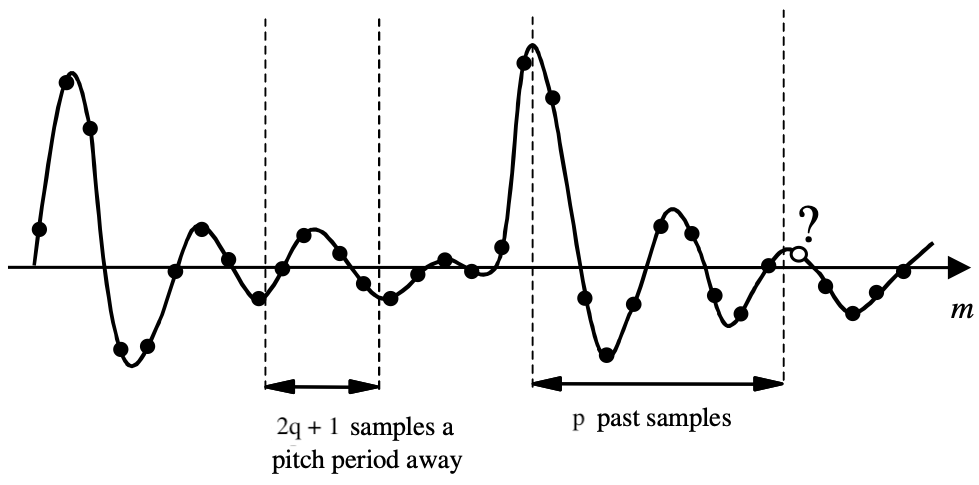
\includegraphics[width=\columnwidth]{shift}
            \caption{Pitch-lag in long-term prediction~\cite{WOS:000266982600001}.}
            \label{fig1}
        \end{figure}
    \end{center}
    \newpage
    %
    \subsection{Reccurent Neural Network}
    %
    In the realm of artificial intelligence and machine learning, recurrent neural networks (RNNs)
    have emerged as powerful tools for modeling and understanding sequential data.
    Unlike traditional feedforward neural networks, RNNs possess the unique ability to capture
    temporal dependencies and dynamic patterns inherent in sequential data, making
    them well-suited for a wide range of applications across various scientific domains.\\
    The ability to comprehend and analyze sequential data is fundamental to understanding the
    dynamics of complex systems in various scientific disciplines. Traditional machine learning
    techniques often struggle to capture the temporal dependencies present in such data,
    hindering their effectiveness in modeling and prediction tasks. Recurrent neural
    networks (RNNs) have emerged as a transformative paradigm for addressing this challenge,
    offering a powerful framework for modeling sequential data with dynamic temporal patterns.
    By introducing feedback loops that enable information to persist over time, RNNs excel
    at processing sequences of data points, making them invaluable tools for scientific research
    across diverse domains.\\
    \\
    \textbf{Architecture and Mechanisms}\\
    At the core of RNNs lies a recurrent structure that allows them to maintain an internal
    state or memory, enabling them to capture long-range dependencies in sequential data. This
    architecture facilitates the processing of input sequences of varying lengths and
    the generation of output sequences with flexible lengths. The key mechanism driving
    RNNs is the recurrent connection, which enables information to flow through the network
    over multiple time steps. Through the use of specialized activation functions such as
    the long short-term memory (LSTM) and gated recurrent unit (GRU), RNNs can effectively
    manage and update their internal states, mitigating the vanishing gradient problem and
    enhancing their ability to capture long-term dependencies.\\
    \\
    The equations of a basic Recurrent Neural Network (RNN) model:\\
    \begin{enumerate}
    \item Hidden State Update
       At each time step \( t \), the hidden state \( h^{(t)} \) of the RNN is updated
       based on the input at the current time step \( x^{(t)} \) and the previous hidden
       state \( h^{(t-1)} \). This update can be represented by the following equation:
       \begin{equation}
        h^{(t)} = \sigma(W_{hx} x^{(t)} + W_{hh} h^{(t-1)} + b_h),
       \end{equation}
       where:\\
       \( h^{(t)} \) is the hidden state at time step \( t \),\\
       \( x^{(t)} \) is the input at time step \( t \),\\
       \( W_{hx} \) is the weight matrix connecting the input to the hidden state,\\
       \( W_{hh} \) is the weight matrix connecting the hidden state to itself (recurrent weights),\\
       \( b_h \) is the bias vector,\\
       \( \sigma \) is the activation function applied element-wise to the input.
    
    \item Output Calculation
       The output \( y^{(t)} \) of the RNN at each time step can be computed based on the
       current hidden state \( h^{(t)} \). This can be represented by the following equation:
       \begin{equation}
        y^{(t)} = \sigma(W_{hy} h^{(t)} + b_y),
       \end{equation}
    
       where:\\
       \( y^{(t)} \) is the output at time step \( t \),\\
       \( W_{hy} \) is the weight matrix connecting the hidden state to the output,\\
       \( b_y \) is the bias vector.
    
    \item Initial Hidden State
       The initial hidden state \( h^{(0)} \) is typically set to a vector of zeros or initialized randomly.
    
    \item Activation Function
       The activation function \( \sigma \) is usually a nonlinear function such as the hyperbolic tangent (tanh) or the rectified linear unit (ReLU).
    
    These equations describe the basic forward pass of a recurrent neural network. During training, the parameters (weights and biases) of the network, \( W_{hx} \), \( W_{hh} \), \( W_{hy} \), \( b_h \), and \( b_y \), are adjusted using backpropagation through time (BPTT) to minimize a specified loss function. This enables the RNN to learn to capture temporal dependencies and make predictions based on sequential data.
    \end{enumerate}
    %
    \subsection{Long short-term memory}
    %
    Long Short-Term Memory (LSTM) networks~\cite{hochreiter1997} are a special kind of Recurrent Neural
    Network (RNN) capable of learning long-term dependencies in sequence prediction
    problems. This is crucial in many deep learning tasks where classical RNNs could fail
    due to the vanishing gradient problem—as gradients are propagated back through the
    network, they can become vanishingly small, effectively preventing the network from
    learning long-range dependencies.\\
    \\
    LSTMs were introduced by Sepp Hochreiter and Jürgen Schmidhuber in 1997
    to specifically address this issue. They incorporate mechanisms called
    gates that regulate the flow of information~\cite{hochreiter1997}.\\
    \\
    \textbf{Structure}
    An LSTM unit typically consists of a cell (which contains the state of
    the network) and three gates:
    \begin{itemize}
    \item Forget gate decides what information is discarded from the cell state.
    \item Input gate decides which values will be updated.
    \item Output gate decides what the next hidden state should be.
    \end{itemize}
    \newpage
    \noindent \textbf{Mathematical Formulations}\\
    \\
    Let's define the following:\\
    \( x_t \): input vector at time step \( t \)\\
    \( h_{t-1} \): hidden state from the previous time step\\
    \( C_{t-1} \): cell state from the previous time step\\
    \( \sigma \): sigmoid activation function\\
    \( \tanh \): hyperbolic tangent activation function\\
    \( W \), \( U \) and \( b \): parameter matrices and vector biases that are learned during training\\
    \\
    The equations governing the forward pass in an LSTM cell are:\\
    \\
    \textbf{Forget Gate}
    \begin{equation}
        f_t = \sigma(W_f \cdot [h_{t-1}, x_t] + b_f)
    \end{equation}

    \noindent This gate decides which information to throw away from the cell state.\\
    \\
    \textbf{Input Gate}
    \begin{equation}
        i_t = \sigma(W_i \cdot [h_{t-1}, x_t] + b_i)
    \end{equation}
    \begin{equation}
        \tilde{C}_t = \tanh(W_C \cdot [h_{t-1}, x_t] + b_C)
    \end{equation}
    The input gate layer decides which values will be updated, and a tanh layer creates a vector of new candidate values, \( \tilde{C}_t \), that could be added to the state.\\
    \\
    \textbf{Cell State Update}
    \begin{equation}
        C_t = f_t \ast C_{t-1} + i_t \ast \tilde{C}_t
    \end{equation}
    The old cell state, \( C_{t-1} \), is updated to the new cell state \( C_t \). The forget gate’s output, multiplied by the previous cell state, decides what to forget, and the input gate’s output, multiplied by the candidate values, decides what new information to add.\\
    \\
    \textbf{Output Gate}
    \begin{equation}
        o_t = \sigma(W_o \cdot [h_{t-1}, x_t] + b_o)
    \end{equation}
    \begin{equation}
        h_t = o_t \ast \tanh(C_t)
    \end{equation}
    The output gate decides what the next hidden state, \( h_t \), should be. The hidden state contains information on previous inputs. The contents of the cell state are shaped by a tanh function to ensure they stay between -1 and 1 and are multiplied by the output of the output gate, so that only the necessary information is passed on.
    LSTMs are designed to avoid the long-term dependency problem, allowing them to remember information for extended periods. Due to their effectiveness, they are widely used in tasks that involve sequences, such as speech recognition, language modeling, and text generation. The unique architecture of LSTMs makes them suited for these kinds of tasks where context from the distant past is crucial for understanding the current element in the sequence.
    %

\newpage

\printbibliography

\end{document}